% From this directory: tectonic robust-pca.tex
% Inputs: ../figures/*.pdf and ../report/generated_results.tex
\documentclass[aspectratio=1610,11pt]{beamer}
\usepackage{amsmath,amssymb,booktabs,graphicx}
% Generated by run_all.py from results/. Edits will be overwritten.
\newcommand{\MatrixSize}{100}
\newcommand{\TrueRank}{5}
\newcommand{\Seed}{43}
\newcommand{\Trials}{5}
\newcommand{\Magnitude}{10}
\newcommand{\Threshold}{1}
\newcommand{\LambdaValue}{0.100}
\newcommand{\PenaltyScale}{0.3}
\newcommand{\StopTolerance}{1\times10^{-7}}
\newcommand{\IterationCap}{5000}
\newcommand{\MainTrialCount}{25}
\newcommand{\CorruptTrialCount}{20}
\newcommand{\CorruptWins}{20}
\newcommand{\GapTrend}{increases at every density step}
\newcommand{\MainConverged}{25}
\newcommand{\NoiseConverged}{15}
\newcommand{\NoiseTrials}{15}
\newcommand{\CleanPca}{1.44\times10^{-15}}
\newcommand{\CleanPcp}{2.81\times10^{-8}}
\newcommand{\EndPca}{2.116}
\newcommand{\EndPcp}{1.67\times10^{-7}}
\newcommand{\MainMinIterations}{2}
\newcommand{\MainMaxIterations}{41}
\newcommand{\MeanPcaMs}{0.79}
\newcommand{\MeanPcpMs}{21.05}
\newcommand{\CleanFalsePos}{0}
\newcommand{\CorruptTotalPos}{18500}
\newcommand{\CorruptFalsePos}{0}
\newcommand{\CorruptFalseNeg}{0}
\newcommand{\PooledPrecision}{1.000}
\newcommand{\PooledRecall}{1.000}
\newcommand{\RepPca}{1.242}
\newcommand{\RepPcp}{7.46\times10^{-8}}
\newcommand{\RepRank}{5}
\newcommand{\RepIterations}{32}
\newcommand{\RepStatus}{converged}
\newcommand{\RepPrimal}{1.82\times10^{-8}}
\newcommand{\RepDual}{8.14\times10^{-8}}
\newcommand{\RepTp}{1000}
\newcommand{\RepFp}{0}
\newcommand{\RepFn}{0}
\newcommand{\NoisePcp}{0.363}
\newcommand{\NoiseFalsePos}{991}
\newcommand{\NoiseFalseNeg}{0}
\newcommand{\NoiseMildIterations}{808.8}
\newcommand{\NoiseHighIterations}{193.6}
\newcommand{\Environment}{Windows 11 on an Intel(R) Core(TM) Ultra 9 275HX CPU. Python 3.14.4, NumPy 2.4.4, SciPy 1.17.1, and Matplotlib 3.10.8.}
\newcommand{\ErrorRows}{%
0\% & $1.44\times10^{-15} \pm 6.02\times10^{-16}$ & $2.81\times10^{-8} \pm 2.64\times10^{-8}$ \\
2\% & $0.496 \pm 0.041$ & $2.90\times10^{-8} \pm 1.31\times10^{-8}$ \\
5\% & $0.885 \pm 0.048$ & $4.90\times10^{-8} \pm 3.48\times10^{-8}$ \\
10\% & $1.330 \pm 0.068$ & $7.86\times10^{-8} \pm 1.96\times10^{-8}$ \\
20\% & $2.116 \pm 0.089$ & $1.67\times10^{-7} \pm 4.64\times10^{-8}$ \\
}
\newcommand{\DiagnosticRows}{%
0\% & $\text{--}$ & 5/5 & 7.2 [2, 9] & 3.6 \\
2\% & $1.000$ & 5/5 & 25.6 [24, 27] & 19.8 \\
5\% & $1.000$ & 5/5 & 27.8 [27, 28] & 23.3 \\
10\% & $1.000$ & 5/5 & 32.2 [30, 35] & 26.4 \\
20\% & $1.000$ & 5/5 & 39.0 [38, 41] & 32.2 \\
}
\newcommand{\NoiseRows}{%
0.0 & $1.391$ & $6.87\times10^{-8}$ & 5.0 & $1.000$ \\
0.1 & $1.391$ & $0.076$ & 54.2 & $1.000$ \\
0.5 & $1.401$ & $0.363$ & 54.8 & $0.910$ \\
}

\graphicspath{{../figures/}}

\definecolor{ink}{HTML}{183447}
\definecolor{muted}{HTML}{4D6170}
\definecolor{accent}{HTML}{155E89}
\setbeamercolor{normal text}{fg=ink,bg=white}
\setbeamercolor{structure}{fg=accent}
\setbeamercolor{frametitle}{fg=ink}
\setbeamercolor{footline}{fg=muted}
\setbeamerfont{frametitle}{size=\Large,series=\bfseries}
\setbeamerfont{footline}{size=\scriptsize}
\setbeamersize{text margin left=8mm,text margin right=8mm}
\setbeamertemplate{navigation symbols}{}
\setbeamertemplate{itemize item}{\raise.18ex\hbox{\scriptsize\textbullet}}
\setbeamertemplate{frametitle}{%
  \vspace*{2.8mm}\usebeamerfont{frametitle}\strut\insertframetitle\par\vspace{1mm}}
\setbeamertemplate{footline}{%
  \leavevmode
  \begin{beamercolorbox}[wd=\paperwidth,ht=3mm,dp=2mm,leftskip=8mm,rightskip=8mm]{footline}
    \usebeamerfont{footline}
    \hfill\insertframenumber\,/\,\inserttotalframenumber
  \end{beamercolorbox}}

\newcommand{\frob}[1]{\left\lVert#1\right\rVert_{\mathrm F}}
\newcommand{\heading}[1]{\textcolor{accent}{\textbf{#1}}\par\smallskip}
\newcommand{\sourcehint}[1]{\vspace{1mm}{\scriptsize\textcolor{muted}{#1}}\par}
\newcommand{\bullets}{\begin{itemize}\setlength{\itemsep}{2.6mm}}
\newcommand{\closeitems}{\end{itemize}}
\newcommand{\shorttitle}{Robust Low-Rank Matrix Recovery Under Sparse Corruptions}
\title{\shorttitle}
\subtitle{A Comparative Study of PCA and Principal Component Pursuit}
\author{Aashish M}

\begin{document}

% 01
\begin{frame}
  \noindent{\small\textcolor{accent}{\textbf{Pattern Recognition and Machine Learning}}}\par
  \vspace{4mm}
  {\fontsize{25}{29}\selectfont\bfseries
    Robust Low-Rank Matrix Recovery\\
    Under Sparse Corruptions\par}
  \vspace{3mm}
  {\large\textcolor{muted}{A Comparative Study of PCA and Principal Component Pursuit}}\par
  \vspace{7mm}
  {\normalsize\insertauthor\par}
\end{frame}

% 02
\begin{frame}[t]{Motivation and hypothesis}
  \begin{columns}[T,onlytextwidth]
    \begin{column}{.49\textwidth}
      \heading{Recovery problem}
      \bullets
        \item Shared structure across samples or features
        \item Sparse, high-amplitude errors in individual entries
        \item Example: persistent video background and localized foreground motion [3]
      \closeitems
    \end{column}
    \begin{column}{.45\textwidth}
      \heading{Study question}
      \bullets
        \item Recovery of the clean matrix and the corruption locations
        \item Comparison with a known-rank SVD baseline on identical inputs
      \closeitems
    \end{column}
  \end{columns}
  \vspace{4mm}
  \heading{H1}
  \bullets
    \item Lower reconstruction error for PCP under incoherent low-rank structure
      and random sparse errors, with a wider advantage at higher corruption density
  \closeitems
\end{frame}

% 03
\begin{frame}[t]{Synthetic data and experiment parameters}
  \[
    \underbrace{M}_{\text{observed}}
    =\underbrace{L_0}_{\text{clean signal}}
    +\underbrace{S_0}_{\text{sparse errors}},
    \qquad
    L_0=\frac{AB^\top}{\sqrt r},
    \quad A_{ik},\,B_{jk}\overset{\mathrm{iid}}{\sim}\mathcal N(0,1).
  \]
  \vspace{1mm}
  \begin{columns}[T,onlytextwidth]
    \begin{column}{.49\textwidth}
      \heading{Signal and corruption}
      \bullets
        \item Matrix size \(\MatrixSize\times\MatrixSize\), true rank \(r=\TrueRank\)
        \item Unit entry variance in \(L_0\) from \(1/\sqrt r\) scaling
        \item \(\operatorname{round}(pmn)\) distinct locations, sampled uniformly
        \item Independent signs, magnitude \(\Magnitude\) at each selected entry
      \closeitems
    \end{column}
    \begin{column}{.45\textwidth}
      \heading{Trial design}
      \bullets
        \item Density \(p\in\{0,2,5,10,20\}\%\)
        \item \(\Trials\) independent draws per density, \(\MainTrialCount\) main trials
        \item Seed \(\Seed\) with separate trial streams
        \item Shared \(M\) per trial for both methods
      \closeitems
    \end{column}
  \end{columns}
\end{frame}

% 04
\begin{frame}[t]{Truncated SVD baseline}
  \[
    M=U\Sigma V^\top,\qquad
    \hat L_{\mathrm{PCA}}=U_r\Sigma_r V_r^\top,\qquad
    \hat L_{\mathrm{PCA}}\in\arg\min_{\operatorname{rank}(L)\le r}\frob{M-L}^{\,2}.
  \]
  \vspace{3mm}
  \bullets
    \item Top \(r=\TrueRank\) singular directions, with the true rank supplied
    \item Optimal squared-error approximation to \(M\) at rank \(r\) [1]
    \item Recovery evaluated against \(L_0\), a different target from the fitted \(M\)
    \item Uncentered SVD for raw matrix recovery
    \item Centered PCA on \(M-\mathbf{1}\bar m^\top\), with the mean restored
      for reconstruction in the original coordinates [2]
  \closeitems
\end{frame}

% 05
\begin{frame}[t]{Principal Component Pursuit}
  \[
    \boxed{\min_{L,S}\ \|L\|_*+\lambda\|S\|_1
    \quad\text{subject to}\quad L+S=M}
    \qquad \lambda=\frac{1}{\sqrt{\max(m,n)}}=\LambdaValue .
  \]
  \vspace{3mm}
  \begin{columns}[T,onlytextwidth]
    \begin{column}{.48\textwidth}
      \heading{Convex penalties}
      \bullets
        \item Nuclear norm \(\|L\|_*=\sum_i\sigma_i(L)\), favoring low rank
        \item Entrywise norm \(\|S\|_1=\sum_{ij}|S_{ij}|\), favoring sparse errors
        \item Rank and corruption locations inferred jointly
      \closeitems
    \end{column}
    \begin{column}{.46\textwidth}
      \heading{Identifiability}
      \bullets
        \item Incoherent signal directions, spread across coordinates
        \item Sufficiently low rank and scattered corruption support
        \item Single-entry matrix as an ambiguous case, both sparse and rank one
      \closeitems
    \end{column}
  \end{columns}
  \sourcehint{PCP formulation and conditional recovery guarantees [3]}
\end{frame}

% 06
\begin{frame}[t]{Scaled ADMM updates}
  \[
    \mathcal L_\mu=
    \|L\|_*+\lambda\|S\|_1+
    \frac{\mu}{2}\frob{M-L-S+Y}^{\,2}
    -\frac{\mu}{2}\frob{Y}^{\,2}.
  \]
  \[
    \begin{aligned}
      L^{k+1} &= \operatorname{SVT}_{1/\mu}\big(M-S^k+Y^k\big),\\
      S^{k+1} &= \operatorname{Soft}_{\lambda/\mu}\big(M-L^{k+1}+Y^k\big),\\
      Y^{k+1} &= Y^k+M-L^{k+1}-S^{k+1}.
    \end{aligned}
  \]
  \bullets
    \item \(L\) step: shrink singular values via \(\sigma\mapsto(\sigma-t)_+\) [4]
    \item \(S\) step: shrink entries via \(z\mapsto\operatorname{sgn}(z)(|z|-t)_+\)
    \item Dual step: accumulate the constraint mismatch [5]
    \item \(S^0=Y^0=0\), fixed \(\mu=\PenaltyScale\sqrt{mn}/\frob{M}\) for nonzero \(M\)
    \item Cap of \(\IterationCap\) iterations
  \closeitems
\end{frame}

% 07
\begin{frame}[t]{Evaluation protocol}
  \begin{columns}[T,onlytextwidth]
    \begin{column}{.48\textwidth}
      \heading{Signal reconstruction}
      \[
        E_L=\frac{\frob{\hat L-L_0}}{\frob{L_0}}.
      \]
      \bullets
        \item Mean and sample SD across \(\Trials\) trials per density
        \item First \(10\%\) trial for the component and residual plots
        \item Solver time, iteration counts, and convergence status
      \closeitems
    \end{column}
    \begin{column}{.47\textwidth}
      \heading{Corruption detection}
      \[
        \hat\Omega=\{(i,j):|\hat S_{ij}|>\Threshold\}.
      \]
      \bullets
        \item Predicted mask against true support \(\Omega\)
        \item Precision, recall, F1, and false-positive rate
        \item Empty true support at \(0\%\): undefined recall and F1, false alarms reported separately
      \closeitems
    \end{column}
  \end{columns}
\end{frame}

% 08
\begin{frame}[t]{Reconstruction error across corruption densities}
  \begin{columns}[c,onlytextwidth]
    \begin{column}{.57\textwidth}
      \centering
      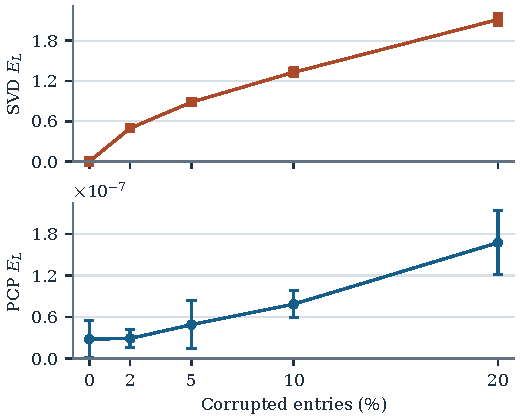
\includegraphics[width=\linewidth,height=66mm,keepaspectratio]{reconstruction_error.pdf}
    \end{column}
    \begin{column}{.39\textwidth}
      \bullets
        \item Clean control: SVD near machine precision
        \item Lower PCP error in \(\CorruptWins/\CorruptTrialCount\) corrupted trials
        \item At \(20\%\): \(\EndPca\) for SVD, \(\EndPcp\) for PCP
        \item Widening mean error gap across the tested sweep
      \closeitems
    \end{column}
  \end{columns}
  \sourcehint{Mean \(\pm\) one sample SD, with separate vertical scales}
\end{frame}

% 09
\begin{frame}[t]{Why the reconstruction errors diverged}
  \begin{columns}[T,onlytextwidth]
    \begin{column}{.66\textwidth}
      \heading{Measured error by density}
      {\small
      \setlength{\tabcolsep}{2.6pt}
      \renewcommand{\arraystretch}{1.32}
      \begin{tabular}{@{}rcc@{}}
        \toprule
        \(p\) & Truncated SVD & PCP\\
        \midrule
        \ErrorRows
        \bottomrule
      \end{tabular}}
      \sourcehint{Relative Frobenius error, mean \(\pm\) sample SD}
    \end{column}
    \begin{column}{.31\textwidth}
      \heading{Corruption energy}
      \[
        \frac{\frob{S_0}}{\sqrt{\mathbb E\frob{L_0}^2}}
        =\Magnitude\sqrt{p}.
      \]
      \bullets
        \item \(1.41\times\) the signal scale at just \(2\%\)
        \item SVD directions pulled toward large errors in \(M\)
        \item PCP allocation of isolated errors to \(S\)
      \closeitems
    \end{column}
  \end{columns}
\end{frame}

% 10
\begin{frame}[t]{Component recovery at 10\% corruption}
  \noindent\makebox[\linewidth][c]{%
    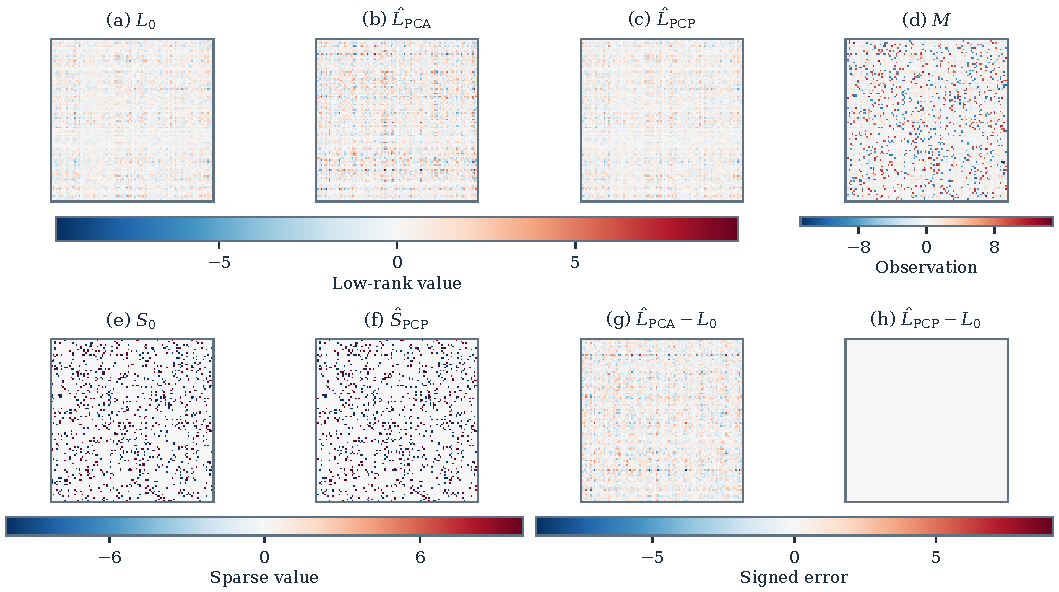
\includegraphics[width=\linewidth,height=61mm,keepaspectratio]{matrix_recovery.pdf}}\par
  \vspace{-1mm}
  \begin{itemize}
    \item Trial 1: \(E_L=\RepPca\) for SVD, \(E_L=\RepPcp\) for PCP, fitted PCP rank \(\RepRank\)
    \item Shared scales for panels (a)--(c), (e)--(f), and (g)--(h)
  \end{itemize}
\end{frame}

% 11
\begin{frame}[t]{Corruption support recovery}
  \begin{columns}[c,onlytextwidth]
    \begin{column}{.49\textwidth}
      \centering
      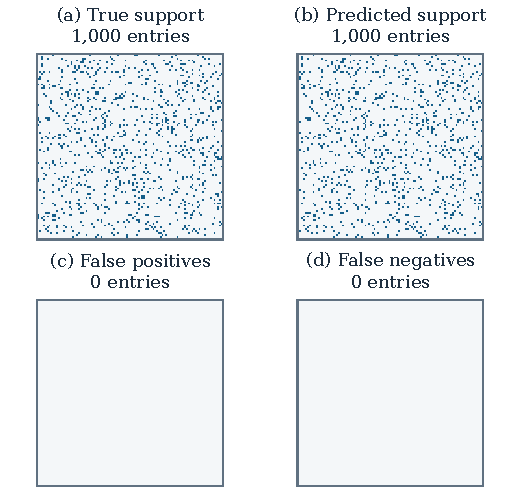
\includegraphics[width=\linewidth,height=68mm,keepaspectratio]{corruption_detection.pdf}
    \end{column}
    \begin{column}{.47\textwidth}
      \heading{\(10\%\) corruption, trial 1}
      \bullets
        \item \(\RepTp\) detections, \(\RepFp\) false positives, \(\RepFn\) misses
        \item Threshold \(|\hat S_{ij}|>\Threshold\) for errors of magnitude \(\Magnitude\)
      \closeitems
      \vspace{3mm}
      \heading{Across the corrupted main trials}
      \bullets
        \item \(\CorruptTotalPos\) true corruptions, \(\CorruptFalsePos\) false positives, \(\CorruptFalseNeg\) misses
        \item Mean F1 of \(1.000\) at each nonzero density
      \closeitems
    \end{column}
  \end{columns}
\end{frame}

% 12
\begin{frame}[t]{Convergence and computational cost}
  \begin{columns}[c,onlytextwidth]
    \begin{column}{.54\textwidth}
      \centering
      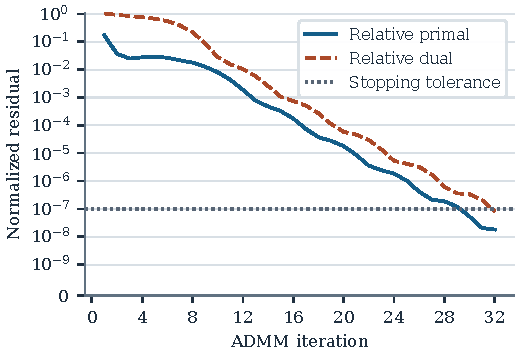
\includegraphics[width=\linewidth,height=61mm,keepaspectratio]{convergence.pdf}
      \sourcehint{\(10\%\) corruption, trial 1, \RepIterations{} iterations}
    \end{column}
    \begin{column}{.43\textwidth}
      \[
        \begin{aligned}
        \rho_{\mathrm p}^{k+1}
           &=\frac{\frob{M-L^{k+1}-S^{k+1}}}{\frob{M}},\\
        \rho_{\mathrm d}^{k+1}
           &=\frac{\mu\frob{S^{k+1}-S^k}}{\max(1,\frob{\mu Y^{k+1}})}.
        \end{aligned}
      \]
      \begin{itemize}
        \setlength{\itemsep}{1.6mm}
        \item Feasibility and stationarity residuals both \(\le\StopTolerance\)
        \item \(\MainConverged/\MainTrialCount\) main runs converged, \(\MainMinIterations\)--\(\MainMaxIterations\) iterations
        \item Mean time: \(\MeanPcaMs\) ms (SVD), \(\MeanPcpMs\) ms (PCP)
        \item One economy SVD per PCP iteration
      \end{itemize}
    \end{column}
  \end{columns}
\end{frame}

% 13
\begin{frame}[t]{Dense Gaussian noise extension}
  \[
    M=L_0+S_0+\sigma Z,\qquad
    Z_{ij}\overset{\mathrm{iid}}{\sim}\mathcal N(0,1),\qquad p=10\%.
  \]
  \begin{columns}[T,onlytextwidth]
    \begin{column}{.52\textwidth}
      \heading{Means across \Trials{} trials per level}
      {\small
      \setlength{\tabcolsep}{4.4pt}
      \renewcommand{\arraystretch}{1.3}
      \begin{tabular}{@{}rcccc@{}}
        \toprule
        \(\sigma\) & SVD \(E_L\) & PCP \(E_L\) & PCP rank & F1\\
        \midrule
        \NoiseRows
        \bottomrule
      \end{tabular}}
      \sourcehint{Shared \(L_0,S_0,Z\) within each trial across all \(\sigma\)}
    \end{column}
    \begin{column}{.44\textwidth}
      \heading{Effect of model mismatch}
      \bullets
        \item Dense noise absorbed into the fitted components under exact equality
        \item \(\NoiseFalsePos\) false positives at \(\sigma=0.5\)
        \item All \(\NoiseConverged/\NoiseTrials\) fits numerically converged
      \closeitems
    \end{column}
  \end{columns}
  \vspace{3mm}
  \bullets
    \item Stable PCP [6]: residual budget \(\frob{M-L-S}\le\varepsilon\) for dense noise
  \closeitems
\end{frame}

% 14
\begin{frame}[t]{Conclusions and scope}
  \begin{columns}[T,onlytextwidth]
    \begin{column}{.48\textwidth}
      \heading{Evidence from the experiment}
      \bullets
        \item H1 supported across the tested sparse corruption sweep
        \item Near-exact PCP signal recovery with accurate support detection
        \item SVD as the faster fit in the clean, known-rank control
        \item Repeated decompositions as the main PCP cost
      \closeitems
    \end{column}
    \begin{column}{.46\textwidth}
      \heading{Limits of the evidence}
      \bullets
        \item Synthetic Gaussian factors and one gross error magnitude
        \item Descriptive comparisons from five trials per density
        \item Coherent signal or clustered errors as sources of ambiguity
        \item Dense noise as a source of higher fitted rank and false alarms
      \closeitems
    \end{column}
  \end{columns}
\end{frame}

% 15
\begin{frame}[t]{References}
  \small
  \begin{itemize}
    \setlength{\itemsep}{3.5mm}
    \item[{[1]}] Eckart and Young, \href{https://doi.org/10.1007/BF02288367}{\emph{The Approximation of One Matrix by Another of Lower Rank}}, 1936
    \item[{[2]}] Jolliffe, \href{https://doi.org/10.1007/b98835}{\emph{Principal Component Analysis}}, 2nd ed., 2002
    \item[{[3]}] Cand\`es, Li, Ma, and Wright, \href{https://doi.org/10.1145/1970392.1970395}{\emph{Robust Principal Component Analysis?}}, 2011
    \item[{[4]}] Cai, Cand\`es, and Shen, \href{https://doi.org/10.1137/080738970}{\emph{A Singular Value Thresholding Algorithm for Matrix Completion}}, 2010
    \item[{[5]}] Boyd et al., \href{https://doi.org/10.1561/2200000016}{\emph{Distributed Optimization and Statistical Learning via the Alternating Direction Method of Multipliers}}, 2011
    \item[{[6]}] Zhou et al., \href{https://doi.org/10.1109/ISIT.2010.5513535}{\emph{Stable Principal Component Pursuit}}, 2010
  \end{itemize}
\end{frame}

\end{document}
